\documentclass[conference]{IEEEtran}
\usepackage{graphicx}
\usepackage{amsmath}
\usepackage{cite}
\usepackage{url}

\title{Eigenfaces for Face Recognition: PCA-Based Analysis on ORL Dataset}
\author{\IEEEauthorblockN{Emircan Sarı}
\IEEEauthorblockA{Istanbul Technical University \\
\texttt{sariem22@itu.edu.tr}}
}

\begin{document}
\maketitle

\begin{abstract}
This project implements the Eigenfaces method for face recognition based on Principal Component Analysis (PCA) using the ORL face dataset. We walk through five stages: preprocessing, PCA and eigenface generation, face reconstruction, classification, and robustness to noise. The results demonstrate the effectiveness of PCA in dimensionality reduction and facial identity encoding.
\end{abstract}

\section{Introduction}
Face recognition is a widely researched topic in computer vision. The Eigenfaces method, introduced by Turk and Pentland \cite{turk1991eigenfaces}, uses PCA to reduce high-dimensional facial image data to a lower-dimensional space while preserving significant identity-relevant features. This paper evaluates the method across five tasks and experiments using the ORL dataset.

\section{Task 1: Data Preprocessing}
All images were resized to \(112 \times 92\) and converted to grayscale vectors. The mean face was calculated for both the entire dataset and a subset of 10 images.

\begin{figure}[htbp]
\centering
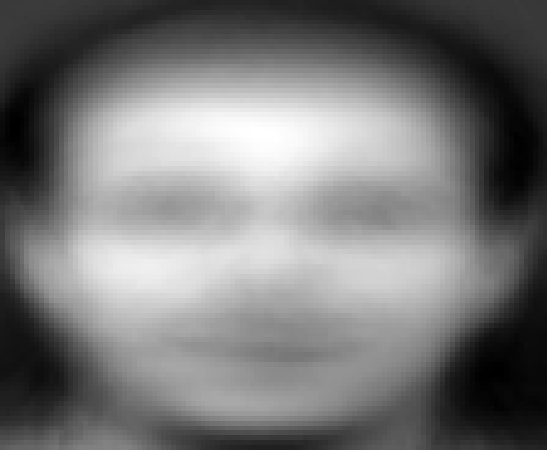
\includegraphics[width=0.4\linewidth]{mean_face_all.png}
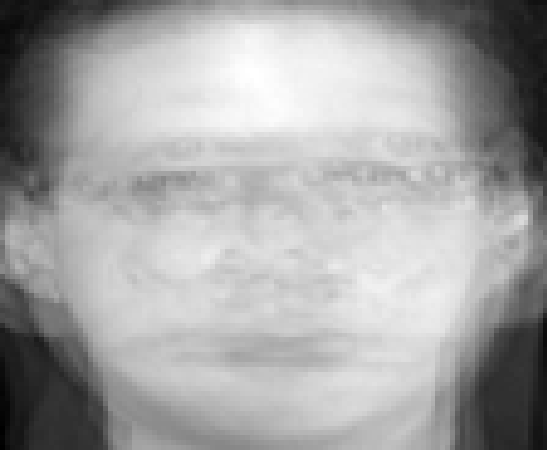
\includegraphics[width=0.4\linewidth]{mean_face_subset.png}
\caption{Mean face from all images (left) vs subset (right)}
\end{figure}

\section{Task 2: PCA and Eigenfaces}
We applied PCA to compute the eigenvectors of the covariance matrix of centered data. These eigenvectors (Eigenfaces) capture the most significant variance directions in the dataset.

\begin{figure}[htbp]
\centering
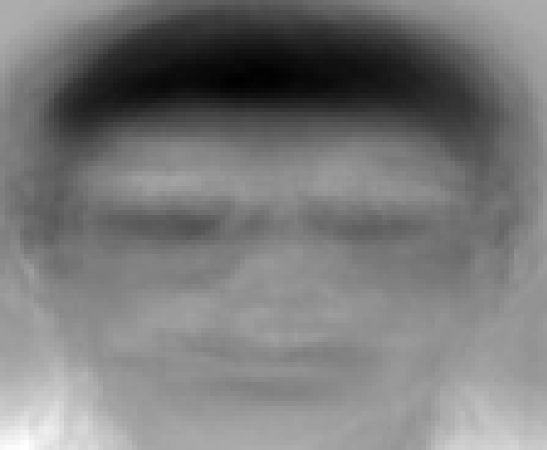
\includegraphics[width=\linewidth]{eigenfaces/ef_0_10.png}
\caption{Top Eigenface (ef\_0\_10.png). Resembles a "ghostly" average face.}
\end{figure}

\begin{figure}[htbp]
\centering
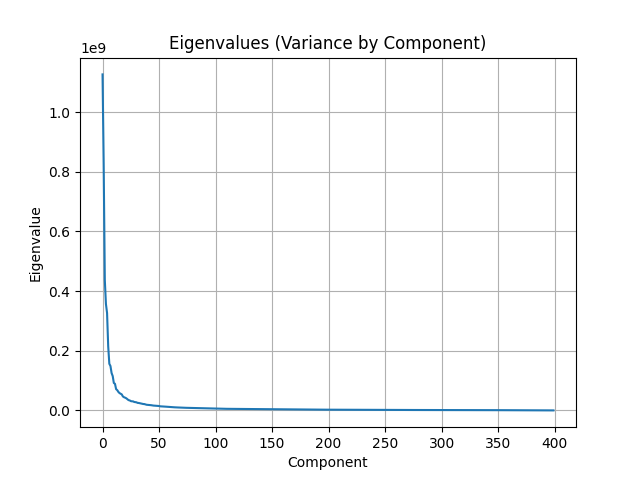
\includegraphics[width=\linewidth]{eigenvalues.png}
\caption{Eigenvalues plotted against principal component index}
\end{figure}

\begin{figure}[htbp]
\centering
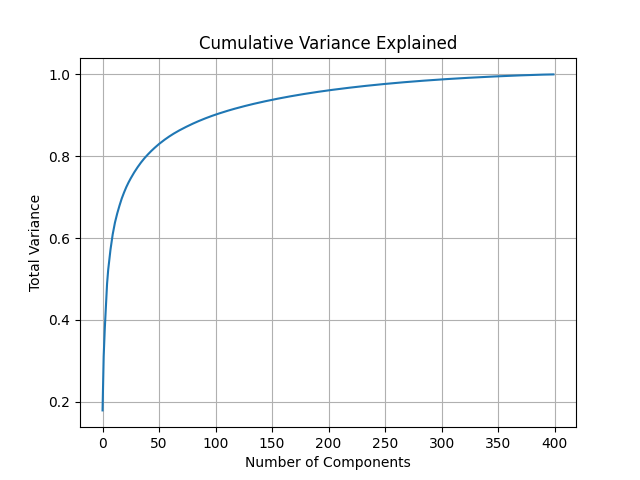
\includegraphics[width=\linewidth]{cumulative_variance.png}
\caption{Cumulative variance: ~95\% achieved with first 100 components}
\end{figure}

\section{Task 3: Face Reconstruction}
Using top \(M\) eigenfaces, we reconstructed original faces for \(s10\) and \(s11\). The quality increases with \(M\), while Mean Squared Error (MSE) decreases.

\begin{figure}[htbp]
\centering
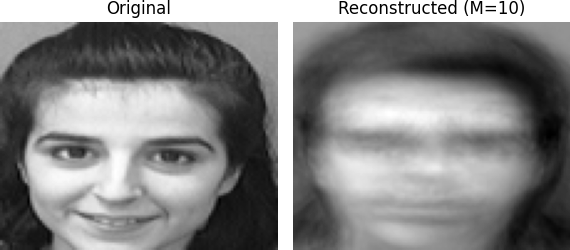
\includegraphics[width=0.9\linewidth]{reconstructed/comparison_10_M10.png}
\caption{Reconstruction with M=10 (left: original, right: blurry)}
\end{figure}

\begin{figure}[htbp]
\centering
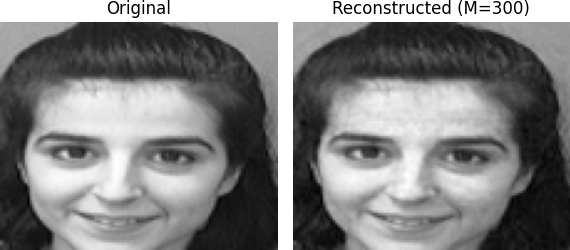
\includegraphics[width=0.9\linewidth]{reconstructed/comparison_10_M300.png}
\caption{Reconstruction with M=300 (right nearly indistinguishable from original)}
\end{figure}

\section{Task 4: Classification with Eigenfaces}
Face recognition was performed using nearest neighbor classification in eigenface space. We achieved up to 98.5\% accuracy.

\begin{figure}[htbp]
\centering
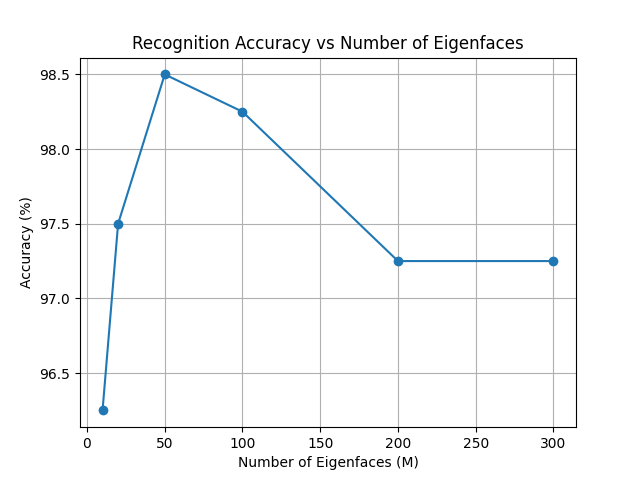
\includegraphics[width=\linewidth]{recognition/accuracy_vs_eigenfaces.png}
\caption{Recognition accuracy vs number of eigenfaces}
\end{figure}

\begin{figure}[htbp]
\centering
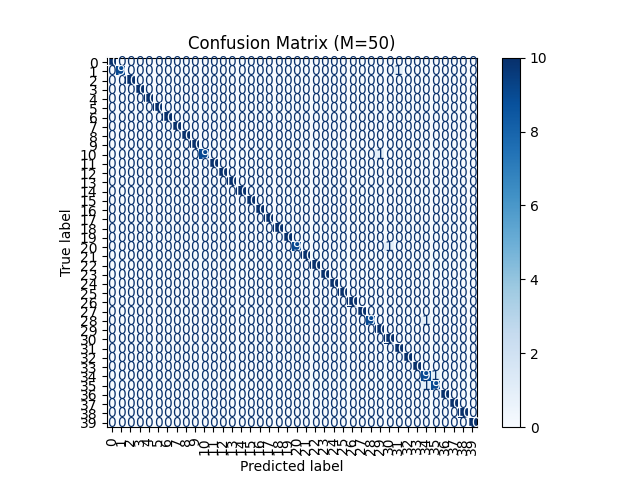
\includegraphics[width=\linewidth]{recognition/confusion_matrix_M50.png}
\caption{Confusion matrix for M=50}
\end{figure}

\section{Task 5: Robustness to Noise}
Recognition accuracy was tested under Gaussian and Salt-and-Pepper noise with M=50. The system showed strong robustness to Gaussian noise up to std=0.5 and to Salt-and-Pepper noise up to 0.4.

\begin{figure}[htbp]
\centering
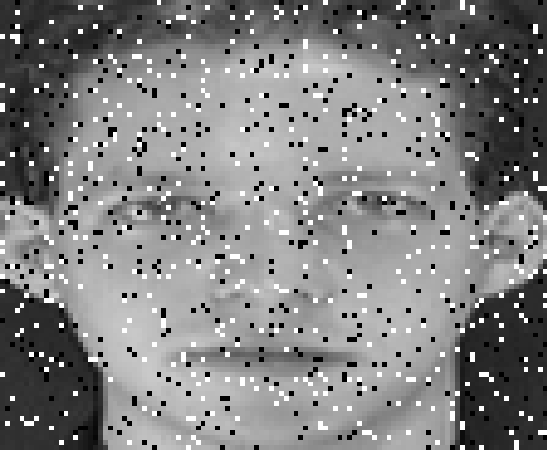
\includegraphics[width=0.48\linewidth]{noise/saltpepper/noisy_salt_01_1.png}
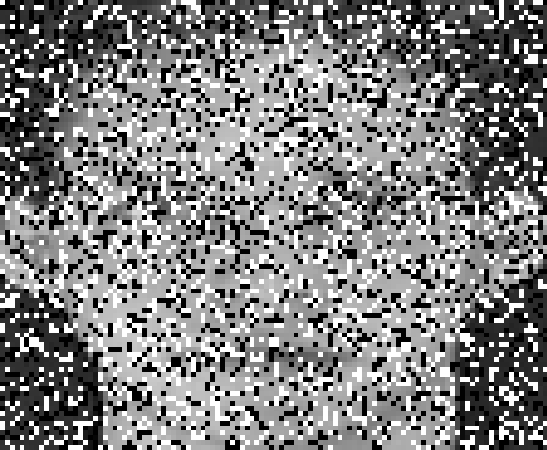
\includegraphics[width=0.48\linewidth]{noise/saltpepper/noisy_salt_05_1.png}
\caption{Salt-and-pepper noise: light (left) vs heavy (right)}
\end{figure}

\begin{figure}[htbp]
\centering
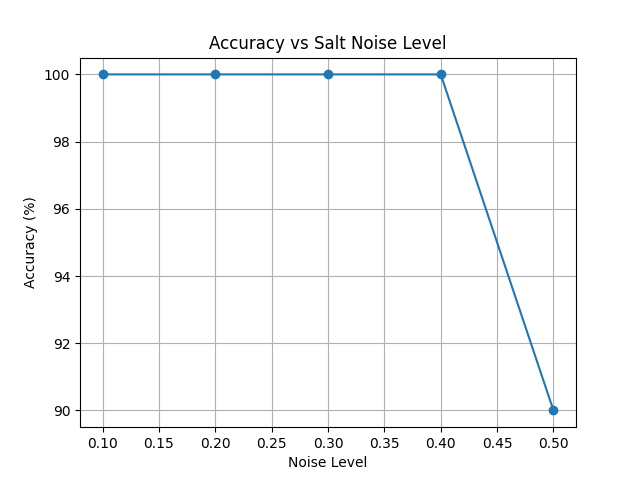
\includegraphics[width=\linewidth]{noise/saltpepper/accuracy_vs_salt_noise.png}
\caption{Accuracy vs Salt-and-Pepper noise level}
\end{figure}

\section{Conclusion}
This project demonstrates that PCA-based Eigenfaces provide a powerful yet simple method for face recognition. The system achieves high recognition accuracy and is resilient to noise. Higher values of \(M\) improve reconstruction and classification but introduce computational costs. An optimal balance around \(M=50\)–100 is often sufficient for practical systems.

\bibliographystyle{IEEEtran}
\bibliography{eigenfaces_refs}

\end{document}
